\chapter{Lab Utilities:实用工具实验}
\begin{introduction}
    \item 启动 xv6
    \item 实现 sleep 工具
    \item 实现 pingpong 工具
    \item 基于管道的质数筛
    \item 进程的基本概念
\end{introduction}

配置好了实验环境后,我们便可以开始进行第一个模块的实验了。Lab Utilities 意为实用工具实验,主要内容是从用户的视角来使用操作系统中的各种特性。

\section{启动 xv6}

上文中我们已经配置好了实验的环境,并将实验的代码库克隆到了本地。在第一个实验的第一个小题中,我们需要编译代码库中的源码并在 qemu 中启动 xv6 系统。

由于 6.S081 已经为 xv6 编写了较为完善的 Makefile ,故而启动 xv6 的过程并不困难。首先,我们需要将实验的代码库切换到 Lab Utilities 的分支,在终端中使用下面的指令:
\begin{lstlisting}
$ cd xv6-labs-2021
$ git checkout util
Branch 'util' set up to track remote branch 'util' from 'origin'.
Switched to a new branch 'util'
\end{lstlisting}
然后,直接使用 \lstinline{make qemu} 即可编译并在 qemu 中运行 xv6 。若一切正常, make 将会执行一系列的编译和链接操作,输出大量的 log ,并且用 qemu 启动 xv6 系统,如下图所示:
\begin{figure}[H]
  \centering
  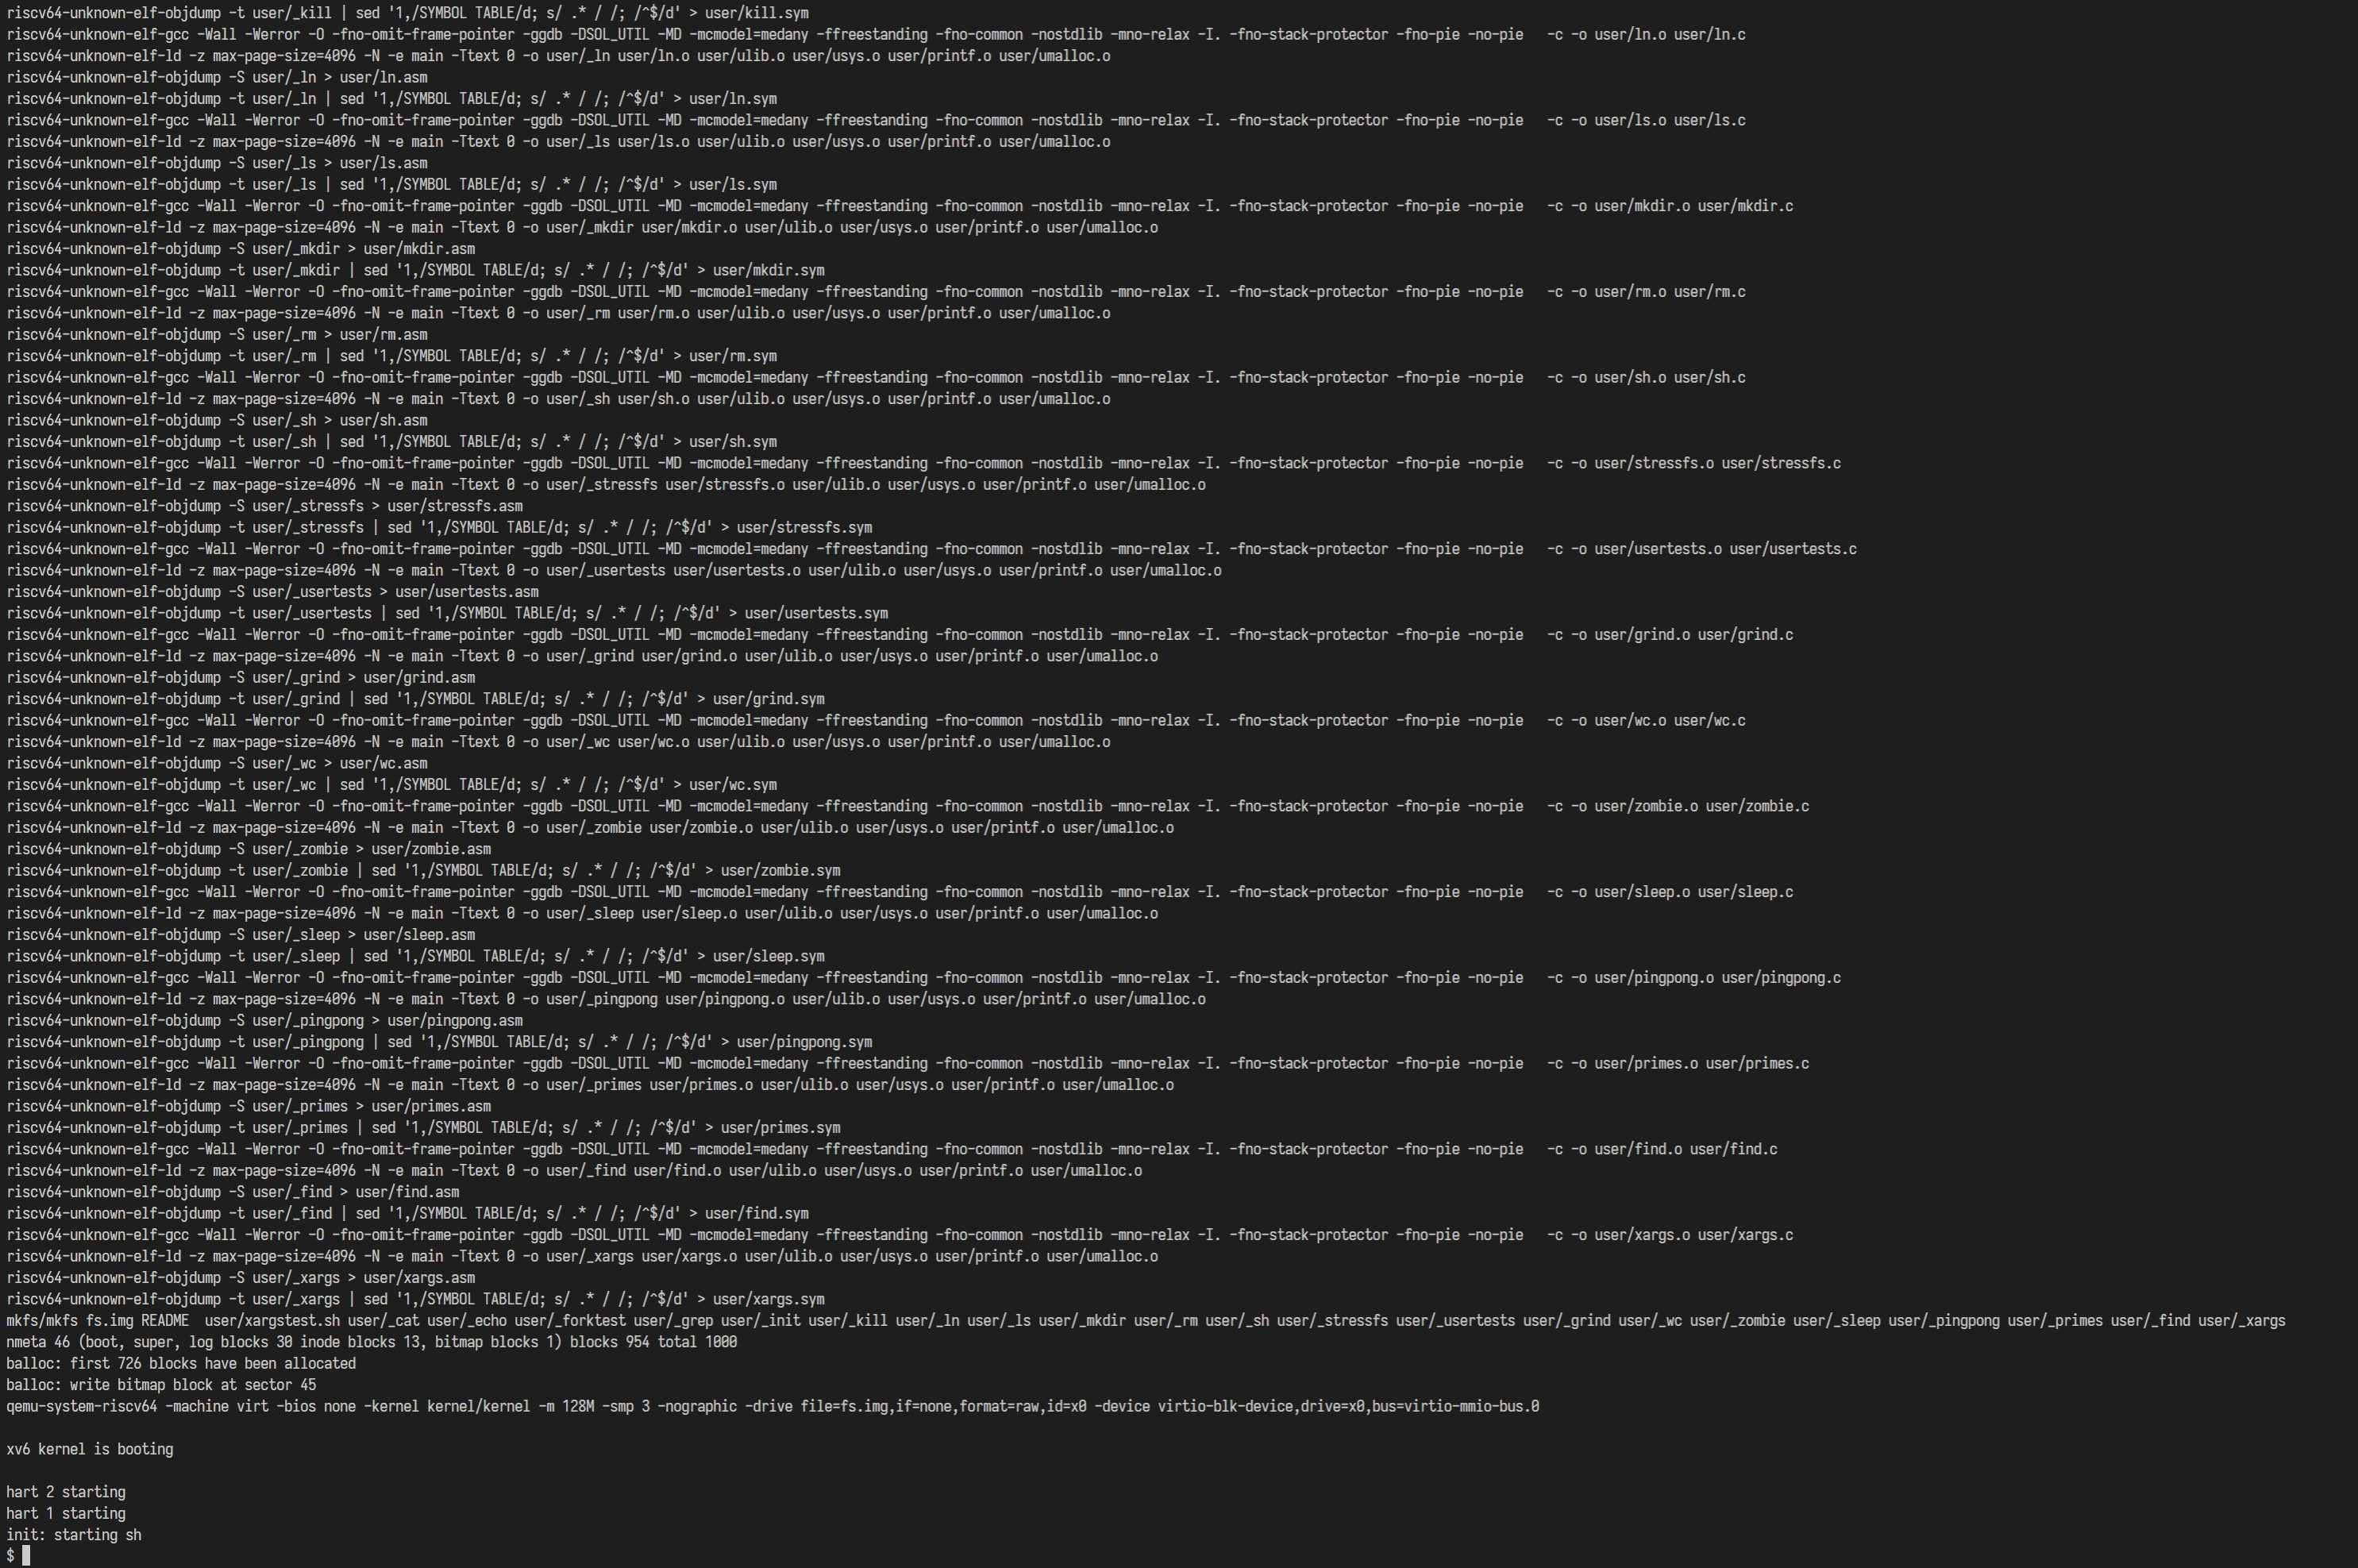
\includegraphics[width=0.7\textwidth]{boot_xv6.jpg}
  \caption{成功启动 xv6 系统的界面}
\end{figure}
xv6 启动后, init 进程会启动一个 shell 等待用户的命令。在这个简易的 shell 中,可以使用 \lstinline{ls} 指令列出根目录下的文件,然后试着执行一些内置的程序,例如执行 \lstinline{cat README} ,即可查看 README 文件的内容。

若要结束运行 xv6 并终止 qemu,需在键盘上同时按下 Ctrl+A 键,然后按下 X 键,即可终止 qemu 的运行。

\section{实现 sleep 工具}

在该实验中,我们需要实现 Unix 中经典的实用工具 sleep 。 sleep 工具的作用是等待给定的 tick 数并退出( tick 是指两次次时钟中断的间隔时间)。根据要求,我们需要将实现的源码放置在 \lstinline{user/sleep.c} 。

在开始写代码之前,我们可以先查看其它实用工具的源码,用以习惯其书写的方式。例如,打开源码 \lstinline{user/echo.c} :
\begin{lstlisting}[language=C]
#include "kernel/types.h"
#include "kernel/stat.h"
#include "user/user.h"

int
main(int argc, char *argv[])
{
  int i;

  for(i = 1; i < argc; i++){
    write(1, argv[i], strlen(argv[i]));
    if(i + 1 < argc){
      write(1, " ", 1);
    } else {
      write(1, "\n", 1);
    }
  }

  exit(0);
}
\end{lstlisting}

注意到该源码与我们日常书写的 C 语言源码大致相同,但也存在几个明显的区别:

1) include 部分引入的头文件不是标准的 C 语言库的头文件(毕竟 xv6 还没有实现标准 C 语言库);

2)程序退出时使用的是 \lstinline{exit(0);} 而非一般的 \lstinline{return 0;} 。

\begin{proposition}[为什么使用 exit 系统调用退出]
实际上,在用 gcc 为 linux 构建程序时,工具链会添加所需的 exit 调用,真正的程序执行并非从 main 函数开始,而是从工具链添加的 start 函数开始的,示意代码如下所示:
\begin{lstlisting}[language=C]
void start(void) {
    /* get argc, argv, env) */
    int r = main(argc, argv, envp);  /*  << start calls the actual main */
    exit(r);
}
\end{lstlisting}
在 xv6 中,由于我们没有这样配置工具链,故而需要手动添加 \lstinline{exit(0);} 语句。
该系统调用的作用是按照既定的步骤结束一个进程(关闭文件,释放资源,唤醒等待的父进程,修改自身状态等),具体实现参照 \lstinline{kernel/proc.c} 中的 \lstinline{void exit(int status)}。
\end{proposition}

熟悉了 \lstinline{user/echo.c} 的写法后,我们将该文件复制为 \lstinline{user/sleep.c} ,然后对其进行修改,应该就能得到所需的实用程序。为了查找我们实现 sleep 功能的系统调用,需要打开 \lstinline{user/user.h} 查看我们可以使用的一些系统调用和函数。不难发现, \lstinline{user/user.h} 中定义了如下系统调用:
\begin{lstlisting}[language=C]
  int sleep(int);
\end{lstlisting}
由于 sleep 只接受一个参数,故而我们可以简化对 \lstinline{int argc, char *argv[]} 的处理,使用 \lstinline{user/user.h} 提供的 \lstinline{int atoi(const char*)} 将第一个参数转化为整数,然后执行 \lstinline{int sleep(int)} 系统调用,最后使用 \lstinline{exit(0);} 退出进程。依据此思路写出的 \lstinline{user/sleep.c} 如下所列:
\begin{lstlisting}[language=C]
#include "kernel/types.h"
#include "kernel/stat.h"
#include "user/user.h"

int main(int argc, char *argv[])
{
    int sec;
    if (argc <= 1)
    {
        printf("usage: sleep [seconds]\n");
        exit(0);
    }
    sec = atoi(argv[1]);
    sleep(sec);
    exit(0);
}
\end{lstlisting}

在完成代码的编写后,需要将该源文件加入到 xv6 的 Makefile 里,这样工具链才会编译我们编写的用户程序。打开 \lstinline{Makefile} ,找到 \lstinline{UPROGS} 环境变量,然后按照其格式,在其后面加入一行:
\begin{lstlisting}
	$U/_sleep\
\end{lstlisting}
保存后在终端里执行 \lstinline{make qemu} ,之前编译的内核不会被重新编译,进入 xv6 后输入 \lstinline{ls} ,可以看到我们的程序已经在文件系统的根目录下了。执行 \lstinline{sleep 1000} ,其行为符合预期。

使用 xv6 实验自带的测评工具测评,在终端里输入 \lstinline{./grade-lab-util sleep} ,即可进行自动评测,如下图所示:
\begin{figure}[H]
  \centering
  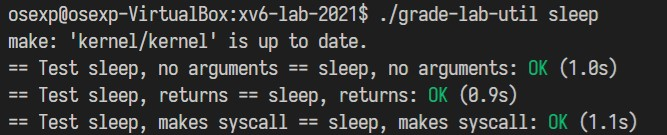
\includegraphics[width=0.8\textwidth]{util_sleep.jpg}
  \caption{ sleep 的测评结果}
\end{figure}
可见测试全部通过。

\section{实现 pingpong 工具}

在该实验中,我们需要实现一个名为 pingpong 的实用工具,用以验证 xv6 的进程通信的一些机制。该程序创建一个子进程,并使用管道与子进程通信:父进程首先发送一字节的数据给子进程,子进程接收到该数据后,在 shell 中打印 "<pid>: received ping" ,其中 pid 为子进程的进程号;子进程接收到数据后,向父进程通过管道发送一字节数据,父进程收到数据后在 shell 中打印 "<pid>: received pong" ,其中 pid 为父进程的进程号。

首先和上一个实验一样,复制一个实用程序的源码到 \lstinline{user/pingpong.c} 并且在 Makefile 中添加该程序。

在开始书写代码之前,我们需要了解实现 pingpong 所需要的系统调用:
\begin{enumerate}
  \item 用于创建管道的 pipe 系统调用
  \item 用于创建子进程的 fork 系统调用
  \item 用于读取管道的 read 系统调用
  \item 用于写管道的 write 系统调用
  \item 用于查询进程号的 getpid 系统调用
\end{enumerate}
此外,\lstinline{user/user.h} 提供了 \lstinline{void printf(const char*, ...)} 函数,用于 shell 中的格式化输出。这些系统调用和函数的作用大多可以通过查看其它已经编写好的用户程序学习,或者可以通过 xv6 的教材 \footnote{\url{https://pdos.csail.mit.edu/6.828/2021/xv6/book-riscv-rev2.pdf}} 进行学习。

根据 pingpong 程序的要求,我们需要先完成创建子进程的工作。一般而言,创建子进程的代码段如下所示:
\begin{lstlisting}[language=C]
    int pid = fork();
    if (pid == 0)
    {
      /*  child process code */
    }
    else
    {
      /*  parent process code */
    }
\end{lstlisting}

这样书写与 fork 系统调用的机制有关: fork 会将父进程的寄存器(又称为上下文)、内存空间和进程控制块复制一份,生成子进程,并且将子进程的进程控制块中的父进程指针指向其父进程;此时父子进程几乎完全一致,为了方便程序判断自己是父还是子, fork 会给两个进程不同的返回值,父进程得到的是子进程的 pid ,而子进程的返回值则为0。通过这个机制,我们便不难理解上面的代码。

在测试完成进程的创建后,我们需要设置管道。考虑到 fork 会将父进程的几乎所有内容完整地复制到子进程中(包括已经赋值完成的变量和打开的文件),我们可以在 fork 前打开两个双向管道,然后分别在父子进程中关闭两个管道的读端和写端,这样就省去了创建完子进程后再进行设置时的种种困难。

有了这些思想,便可以实现出下面的 \lstinline{user/pingpong.c} 的代码:
\begin{lstlisting}[language=C]
#include "kernel/types.h"
#include "kernel/stat.h"
#include "user/user.h"

char buf[128];

int main(int argc, char *argv[])
{
    int p1[2], p2[2], pid;
    pipe(p1);
    pipe(p2);

    if (fork() == 0)
    {
        close(p2[1]);
        close(p1[0]);
        pid = getpid();
        int num_read = read(p2[0], buf, 1);
        if (num_read == 1)
        {
            printf("%d: received ping\n", pid);
            write(p1[1], buf, 1);
        }
    }
    else
    {
        close(p1[1]);
        close(p2[0]);
        pid = getpid();
        write(p2[1], buf, 1);
        int num_read = read(p1[0], buf, 1);
        if (num_read == 1)
        {
            printf("%d: received pong\n", pid);
        }
    }

    exit(0);
}
\end{lstlisting}

保存后在终端里执行 \lstinline{make qemu} ,之前编译的内核不会被重新编译,进入 xv6 后输入 \lstinline{pingpong} ,其打印的内容符合预期。

使用 xv6 实验自带的测评工具测评,在终端里输入 \lstinline{./grade-lab-util pingpong} ,即可进行自动评测,如下图所示:
\begin{figure}[H]
  \centering
  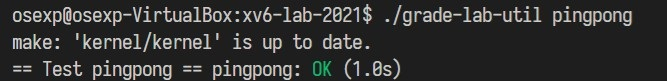
\includegraphics[width=0.8\textwidth]{util_pingpong.jpg}
  \caption{ pingpong 的测评结果}
\end{figure}
可见测试全部通过。

\begin{proposition}[管道的本质]
从我们读写管道使用的 read 和 write 系统调用中不难发现,管道本质上是一种(用于进程间通信缓冲的)特殊的文件。

现实的 Linux 系统中,有大量实用工具只从标准输入读入,并输出到标准输出。考虑到管道其实是一种特殊的文件, shell 可以通过重定向的技术,将标准输入输出重定向到管道中,从而使得这些程序可以用类似流水线的方式串联起来合作完成任务:
\begin{lstlisting}
$ ls user | grep ping
_pingpong
pingpong.asm
pingpong.c
pingpong.d
pingpong.o
pingpong.sym
\end{lstlisting}

上面的例子中,使用“|”连接两个程序: ls 的输出内容流入到管道的一端 (标准输出)。随后,内容一直流到管道的另一端 (标准输入) 由 grep 接收。由于管道本质上是文件,故只接受 byte stream,且可以作为一个固定大小的缓冲区(在 Linux 中默认为 128KB)。在 xv6 中,管道的机制也是类似的。
\end{proposition}


\section{基于管道的质数筛}

通过上面两个实验,我们已经基本熟悉了进程和管道的一些基本概念。这些概念可以帮助我们构建更加高效的、涉及多个进程的程序。一个经典的案例是 Doug McIlroy 提出的基于管道的多进程质数筛 \footnote{原文参见: \url{https://swtch.com/~rsc/thread/}}。

该质数筛的基本思路是每一个进程负责检验一个质数是否为输入的因子,在每次发现一个新质数后,就新建一个进程并令其负责检验该质因子,进程间通过管道传递数据。具体的伪代码如下:
\begin{lstlisting}
p = get a number from left neighbor
print p
loop:
    n = get a number from left neighbor
    if (p does not divide n)
        send n to right neighbor
\end{lstlisting}

最初的父进程负责产生 2 到 maxn 的整数,然后产生一个子进程用于检验质因子 2 。第一个不能被质因子整除的数用于产生下一个子进程,并输出该数,且质数筛的性质保证了该数为质数。

实现过程中,需要维护读端和写端的管道,不断读取上一个进程写入管道的内容,并在合适的条件下生成子进程并将其它数字写入管道。笔者的实现为了简洁,使用了主函数递归来避免多次的 fork 调用:
\begin{lstlisting}[language=C]
#include "kernel/types.h"
#include "kernel/stat.h"
#include "user/user.h"

const int MAX_NUM = 35;

int p1[2], fdr, fdw;
long p, n;
int is_first = 1;

int main(int argc, char *argv[])
{
    if (is_first == 1)
    {
        is_first = 0;
        pipe(p1);
        fdr = p1[0];
        fdw = p1[1];
        for (n = 2; n <= MAX_NUM; n++)
        {
            write(fdw, (void *)&n, 8);
        }
        close(fdw);
    }
    if (fork() == 0)
    {
        if (read(fdr, (void *)&p, 8))
        {
            printf("prime %d\n", p);
            pipe(p1);
            fdw = p1[1];
        }

        while (read(fdr, (void *)&n, 8))
        {
            if (n % p != 0)
                write(fdw, (void *)&n, 8);
        }
        fdr = p1[0];
        close(fdw);
        main(argc, argv);
    }
    else
    {
        wait((int *)0);
        close(fdr);
    }

    exit(0);
}
\end{lstlisting}

使用 xv6 实验自带的测评工具测评,在终端里输入 \lstinline{./grade-lab-util primes} ,即可进行自动评测,如下图所示:
\begin{figure}[H]
  \centering
  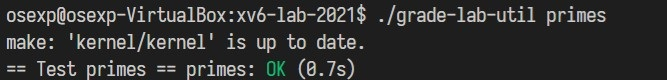
\includegraphics[width=0.8\textwidth]{util_primes.jpg}
  \caption{ primes 的测评结果}
\end{figure}
可见测试全部通过。

\paragraph*{实验结果} 在完成 Lab Utilities 中的所有实验后,根据 MIT 6.S081 的传统,需要在实验目录下创建一个名为 \lstinline{time.txt} 文本文件,其中只包含一行,为完成该实验的小时数。然后在终端中执行 \lstinline{./grade-lab-util} ,即可对整个实验进行自动评分,笔者的结果如下:
\begin{figure}[H]
  \centering
  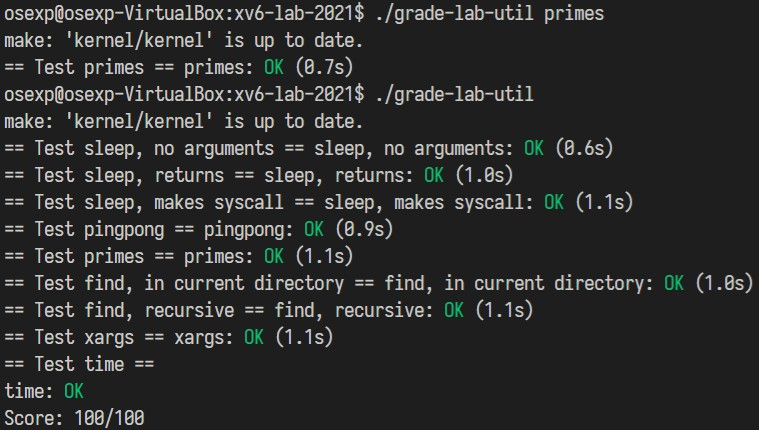
\includegraphics[width=0.8\textwidth]{util_grade.jpg}
  \caption{ Lab Utilities 的测评结果}
\end{figure}
可见测试全部通过,得分为满分。

\section{小结:进程的基本概念}

通过 Lab Utilities 中的几个实验,即便我们没有查阅或修改 xv6 的内核,只是从用户的角度使用进程,也可以如管中窥豹般看到进程的一些性质。

进程作为实例化的程序,拥有自己的地址空间和上下文。这个特点在 pingpong 实验中体现地极为明显:设置好的变量在 fork 之后被保持,且 fork 后的进程中变量的修改不影响原有进程。

进程拥有自己的地址空间和上下文的特点对于并发执行和资源分配是极其有利的,但对于进程间通信则不太友好:相比于直接使用共享内存而言,进程需要借助一种特殊的文件“管道”来进行通信。当进程创建管道时,每次都需要提供两个文件描述符来操作管道。其中一个对管道进行写操作,另一个对管道进行读操作。对管道的读写与一般的 IO 系统函数一致,使用 write 函数写入数据,使用 read 读出数据。

即便 fork 和 pipe 机制十分简明易懂,这两个机制仍然足够让我们构建高效的、涉及多个进程的并发程序。相比于单个进程,多个进程通过管道通信可以有效地利用多 CPU 系统的资源,且配合操作系统的调度可以使得 IO 效率与 CPU 利用率达到较高的水平,从而提高计算机系统的效率。